\documentclass[fleqn,11pt]{wlscirep}
\usepackage[utf8]{inputenc}
\usepackage[T1]{fontenc}
\usepackage{physics}
\usepackage{subfigure}
\usepackage{amsfonts}
\usepackage{amsmath}
\usepackage{amssymb}
\usepackage{mathtools}
\usepackage{bm}
\usepackage{siunitx}
\usepackage{mathptmx}
\usepackage{hyperref}
% Color package
\usepackage{xcolor}
\DeclareSymbolFont{epsilon}{OML}{ntxmi}{m}{it}
\DeclareMathSymbol{\epsilon}{\mathord}{epsilon}{"0F}
% \bibliographystyle{naturemag}
\usepackage[bitstream-charter,cal=cmcal]{mathdesign}

\newcommand{\Ai}{\operatorname{Ai}}
\newcommand{\Bi}{\operatorname{Bi}}

% Meta Data
\title{Non-equilibrium Transitions in Sub/Second Harmonic Generation: Quantum Theory}

\author[1,*]{Kosala Herath}

\affil[1]{Advanced Computing and Simulation Laboratory (A$\chi$L), Department of Electrical and Computer Systems Engineering, Monash University, Clayton, Victoria 3800, Australia}

\affil[*]{kosala.herath@monash.edu}

%\keywords{Keyword1, Keyword2, Keyword3}

\begin{abstract}

{
  This article provides a condensed summary and replication of numerical results from a prior theoretical investigation by Drummond \textit{et al.} \cite{drummond1981} on a non-linear optical system with a mode coupled to its second harmonic. Within this study, a quantum statistical analysis of coherently driven sub/second harmonic generation within an optical resonator is described. Quantum fluctuations are analyzed through a Fokker-Planck equation employing a generalized Glauber-Sudarshan P-representation. Specifically, the analysis focuses on the fluctuation behavior proximate to instability points as predicted by semiclassical theory. Remarkably, the spectrum of the sub-harmonic field exhibits critical narrowing in close proximity to the threshold, indicative of a second-order phase transition. Additionally, at higher driving field intensities, the sub-harmonic spectrum separate into two distinct peaks. Furthermore, the second harmonic light spectrum demonstrates a similar separation below the threshold for hard mode oscillations. Notably, under certain conditions, the photon statistics of the emitted light may reveal photon antibunching phenomena. This understanding and manipulation of anti-bunched light are crucial for advancing various applications in quantum technology, including secure communication, computing, metrology, and imaging.
}

\end{abstract}

\begin{document}

\flushbottom
\maketitle

\thispagestyle{empty}

\section*{Introduction}

The advent of the laser in 1960 \cite{maiman1960} marked a significant milestone, introducing a coherent, high-intensity light source capable of probing matter with unprecedented precision \cite{franken1963}. This breakthrough also initiated a new era in optics, where man-made light fields could apply sufficiently strong electric fields to modify fundamental electronic and optical properties of materials, paving the way for the emergence of non-linear optics \cite{bloembergen2000}.
The utilization of high-intensity lasers enables the exploration of optical non-linearities in materials, offering intriguing prospects for research and applications. Specifically, the investigation of harmonic generation, which involves both upconversion and downconversion frequencies, is pivotal within the realm of non-linear optics. The broad spectrum of applications for harmonic generation extends from contemporary photonics to the analysis and visualization of matter through spectroscopy and microscopy \cite{saleh2019,levenson2012,campagnola2002}.

Second harmonic generation, also known as frequency doubling, occurs when input photons interact with a nonlinear material and effectively combine to produce output photons with twice the frequency of the input photons. Conversely, subharmonic generation is a process where input photons divide to generate output photons with half the frequency of the input field \cite{franken1963,wang2023}. The theoretical analysis conducted by Drummond \textit{et al.} \cite{drummond1981} delved into sub-second harmonic generation within a coherently driven optical cavity, employing a comprehensive quantum mechanical framework. This investigation have described the possibility of non-classical statistics or photon antibunching in non-linear optical processes. While prior studies have addressed these quantum phenomena \cite{stoler1974,mostowski1978}, they  only focused on interacting modes not coupled to an external field, primarily considering transient situations. However, Drummond \textit{et al.} \cite{drummond1981} considered a non-linear crystal situated inside a driven optical cavity, thereby enabling the exploration of steady-state modes.

This review begins by outlining the system model and providing a quantum mechanical description, including the Hamiltonian for the non-linear optical process, which couples lower frequency electromagnetic field modes to higher frequency ones. Following standard procedure and employing the Markov approximation for the thermal baths \cite{louisell1973,walls2008}, the Hamiltonian is transformed into a master equation. Subsequently, by utilizing the Fokker-Plank equation in the complex P-representation \cite{drummond1980}, exact steady-state solutions are be derived. 

\section*{Theoretical Formalism}

In this investigation, we examine the dynamics of a non-linear crystal featuring a second-order susceptibility, situated within a Fabry-Perot interferometer configuration. Our focus lies on the interaction between two distinct light modes characterized by frequencies $\omega_1$ and $\omega_2$. We operate under the assumption that the frequency of the second light mode is approximately twice that of the first, $\omega_2 \approx 2\omega_1$. Both modes are subjected to external coherent phase-locked driving fields oscillating at frequencies $\omega_p$ and $2\omega_p$. This setup enables us to describe the mistuning with respect to the cavity resonance. Moreover, we account for mode damping resulting from cavity losses. Figure \ref{fig_system} presents a schematic representation of the resonant second-order non-linear optical system discussed herein. 
\begin{figure}[!t]
	\centering
	\subfigure{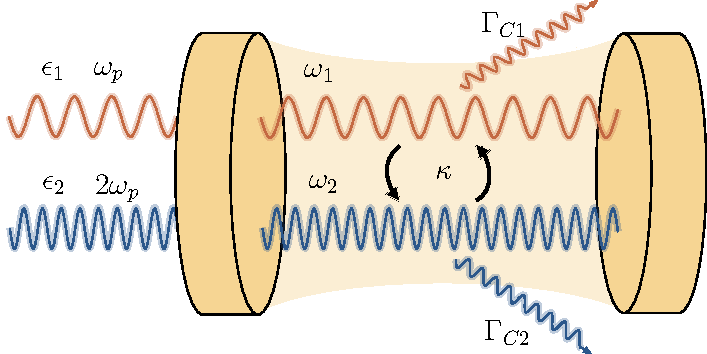
\includegraphics[width=0.5\textwidth]
	  {./figures/system.pdf}}
	\caption{The system comprises a cavity possesses two resonant light modes with frequencies $\omega_1$ and $\omega_2 \approx 2\omega_1$. External coherent driving fields with frequencies $\omega_p$ and $2\omega_p$ are applied to the system. The amplitude of each coherent driving field is denoted by $\epsilon_1$ and $\epsilon_2$. The operators $\hat{\Gamma}{c1}$ and $\hat{\Gamma}{c2}$ represent the heat bath annihilation operators characterizing the cavity losses associated with the two light modes. Furthermore, $\kappa$ is the coupling constant for the interaction between the two light modes.}
	\label{fig_system}
\end{figure}

The interacting Hamiltonian for the describing the system can be written as
\begin{equation}
	\hat{H} = \hat{H}_{\text{cav}} + \hat{H}_{\text{int}} + \hat{H}_{\text{pump}} + \hat{H}_{\text{bath}},
\end{equation}
where the Hamiltonian for the lights modes in the cavity is 
\begin{equation}
	\hat{H}_{\text{cav}} = \hbar\omega_1 \hat{a}_1^{\dagger}\hat{a}_1 +
	\hbar\omega_2 \hat{a}_2^{\dagger}\hat{a}_2,
\end{equation}
the interaction Hamiltonian is
\begin{equation}
	\hat{H}_{\text{int}} = i\hbar \frac{\kappa}{2}
	(\hat{a}_1^{\dagger\;2}\hat{a}_2 +
	\hat{a}_1^2\hat{a}_2^{\dagger}),
\end{equation}
the pumping Hamiltonian is
\begin{equation}
	\hat{H}_{\text{pump}} = 
	i\hbar(
		\epsilon_1\hat{a}_1^{\dagger}\exp(-i\omega_p t) - 
		\epsilon_1^{*}\hat{a}_1\exp(i\omega_p t)
	)
	+ i\hbar(
		\epsilon_2\hat{a}_2^{\dagger}\exp(-2i\omega_p t) - 
		\epsilon_2^{*}\hat{a}_2\exp(2i\omega_p t)
	),
\end{equation}
and the thermal bath Hamiltonian is
\begin{equation}
	\hat{H}_{\text{bath}} = 
	(\hat{a}_1 \hat{\Gamma}_{c1}^{\dagger} + \hat{a}_1^{\dagger}\hat{\Gamma}_{c1}) 
	+
	(\hat{a}_2 \hat{\Gamma}_{c2}^{\dagger} + \hat{a}_2^{\dagger}\hat{\Gamma}_{c2}).
\end{equation}
In this context, $\hat{a}_1$ and $\hat{a}_2$ represents the boson annihilation operators for the modes of frequency $\omega_1$ and $\omega_2$ respectively, $\kappa$ is the coupling contact for the light mode interaction. Moreover, the amplitude of the external driving field is denoted by $\epsilon_1$, and $\hat{\Gamma}{c1}$ and $\hat{\Gamma}{c2}$ represent the heat bath annihilation operators characterizing the cavity losses associated with the two light modes.

Following the standard procedures and tracing out the effects of the bath reservoirs \cite{louisell1973,walls2008}, the equation governing the density operator $\hat{\rho}$ of the two cavity modes can be found as 
\begin{equation}
	\begin{aligned}
		\pdv{\rho}{t} =&
			\frac{1}{i\hbar} [(\hat{H}_{\text{cav}} + \hat{H}_{\text{int}} + \hat{H}_{\text{pump}}),\hat{\rho}] +
			\gamma_1(2\hat{a}_1\hat{\rho}\hat{a}_1^{\dagger} - 
			\hat{a}_1^{\dagger}\hat{a}_1\hat{\rho}
			-\hat{\rho}\hat{a}_1^{\dagger}\hat{a}_1) +
			\gamma_2(2\hat{a}_2\hat{\rho}\hat{a}_2^{\dagger} - 
			\hat{a}_2^{\dagger}\hat{a}_2\hat{\rho}
			-\hat{\rho}\hat{a}_2^{\dagger}\hat{a}_2) \\
			&+ 2\gamma_1n^{\text{th}}_1
			(\hat{a}_1^{\dagger}\hat{\rho}\hat{a}_1 + 
			\hat{a}_1\hat{\rho}\hat{a}_1^{\dagger} -
			\hat{a}_1^{\dagger}\hat{a}_1\hat{\rho}-
			\hat{\rho}\hat{a}_1\hat{a}_1^{\dagger})
			+ 2\gamma_2n^{\text{th}}_2
			(\hat{a}_2^{\dagger}\hat{\rho}\hat{a}_2 + 
			\hat{a}_2\hat{\rho}\hat{a}_2^{\dagger} -
			\hat{a}_2^{\dagger}\hat{a}_2\hat{\rho}-
			\hat{\rho}\hat{a}_1\hat{a}_2^{\dagger}),
	\end{aligned}
\end{equation}
where $\gamma_1$ and $\gamma_2$ are the modes damping constants, and $n^{\text{th}}_1$ and $n^{\text{th}}_2$ are the thermal photon numbers of the baths. This master equation may be solved by various techniques \cite{louisell1973}. However, in this analysis we convert it to an associated $\mathcal{C}$-number equation. We map the master equation to $\mathcal{C}$-number Fokker-Planck
equation in the generalized P representation \cite{walls2008} making the mapping: $(\hat{a}_1,\hat{a}_1^{\dagger},\hat{a}_2,\hat{a}_2^{\dagger}) \leftrightarrow ({\alpha}_1,{\alpha}_1^{+},{\alpha}_2,{\alpha}_2^{+})$. Then, we can identify that 
\begin{equation}
	\begin{aligned}
		\pdv{P(\boldsymbol{\alpha})}{t} =
		\Bigg\{&
			\pdv{\alpha_1}[(\gamma_1 + i\Delta_1)\alpha_1 - \epsilon_1 - \kappa\alpha_1^+\alpha_2]
			+
			\pdv{\alpha_1^+}[(\gamma_1 - i\Delta_1)\alpha_1^+ - \epsilon_1^* - \kappa\alpha_1\alpha_2^+]
			\\
			&\pdv{\alpha_2}[(\gamma_2 + i\Delta_2)\alpha_2 - \epsilon_2 + \frac{\kappa}{2}\alpha_1^2]
			+
			\pdv{\alpha_2^+}[(\gamma_2 - i\Delta_2)\alpha_2^+ - \epsilon_2^* + \frac{\kappa}{2}\alpha_1^{+\;2}]
			\\
			& \frac{1}{2}
			\Bigg[
				\pdv[2]{\alpha_1}(\kappa\alpha_2) 
				+ \frac{\partial^2}{\partial\alpha_1^{+\;2}}(\kappa\alpha_2^+)
				+ 2\gamma_1n^{\text{th}}_1\frac{\partial^2}{\partial\alpha_1\alpha_1^+}
				+ 2\gamma_2n^{\text{th}}_2\frac{\partial^2}{\partial\alpha_2\alpha_2^+}
			\Bigg]
		\Bigg\}P(\boldsymbol{\alpha}),
	\end{aligned}
\end{equation}
where $\boldsymbol{\alpha} = [{\alpha}_1,{\alpha}_1^{+},{\alpha}_2,{\alpha}_2^{+}]^{\intercal}$, $\Delta_1 = \omega_1 - \omega_p$ and $\Delta_2 = \omega_2 - 2\omega_p$. Furthermore, it is important to mention that the following transformation to the rotating frames of the driving fields has been mode in the previous derivation:
\begin{equation}
	\alpha_1 \rightarrow \alpha_1\exp(-i\omega t), \quad \text{and} \quad
	\alpha_2 \rightarrow \alpha_2\exp(-2i\omega t).
\end{equation}
This enables us to establish equivalent stochastic differential equations employing the It$\hat{o}$ rules
\begin{equation}
	\pdv{t}\mqty(\alpha_1 \\ \alpha_1^+)
\end{equation}


































\bibliography{manuscript}

\end{document}
